\problemname{Öar}
2020 års International Olympiad in Informatics (IOI) kommer att avgöras i Singapore, ett till ytan litet land som består av massor av öar. På en av utflykterna på IOI ska de $N$ deltagarna besöka dessa öar. Men deltagarna går och tänker på hur de ska implementera Fibonacci-heapar, så en efter en går vilse och hittar inte tillbaka.

På första ön försvinner en deltagare, på andra ön försvinner ytterligare en deltagare. På var och en av de följande öarna försvinner lika många deltagare som sammanlagt försvann på de två senaste öarna (om inte deltagarna är slut innan dess).

På vilken ö försvinner den sista deltagaren?

\section*{Indata}
Den första raden innehåller ett heltal $1\le N \le 10\,000$, antalet deltagare.

\section*{Utdata}
Ett heltal $A$, numret på ön där den $N$:te deltagaren försvinner.

\begin{figure}[h]
  \centering
      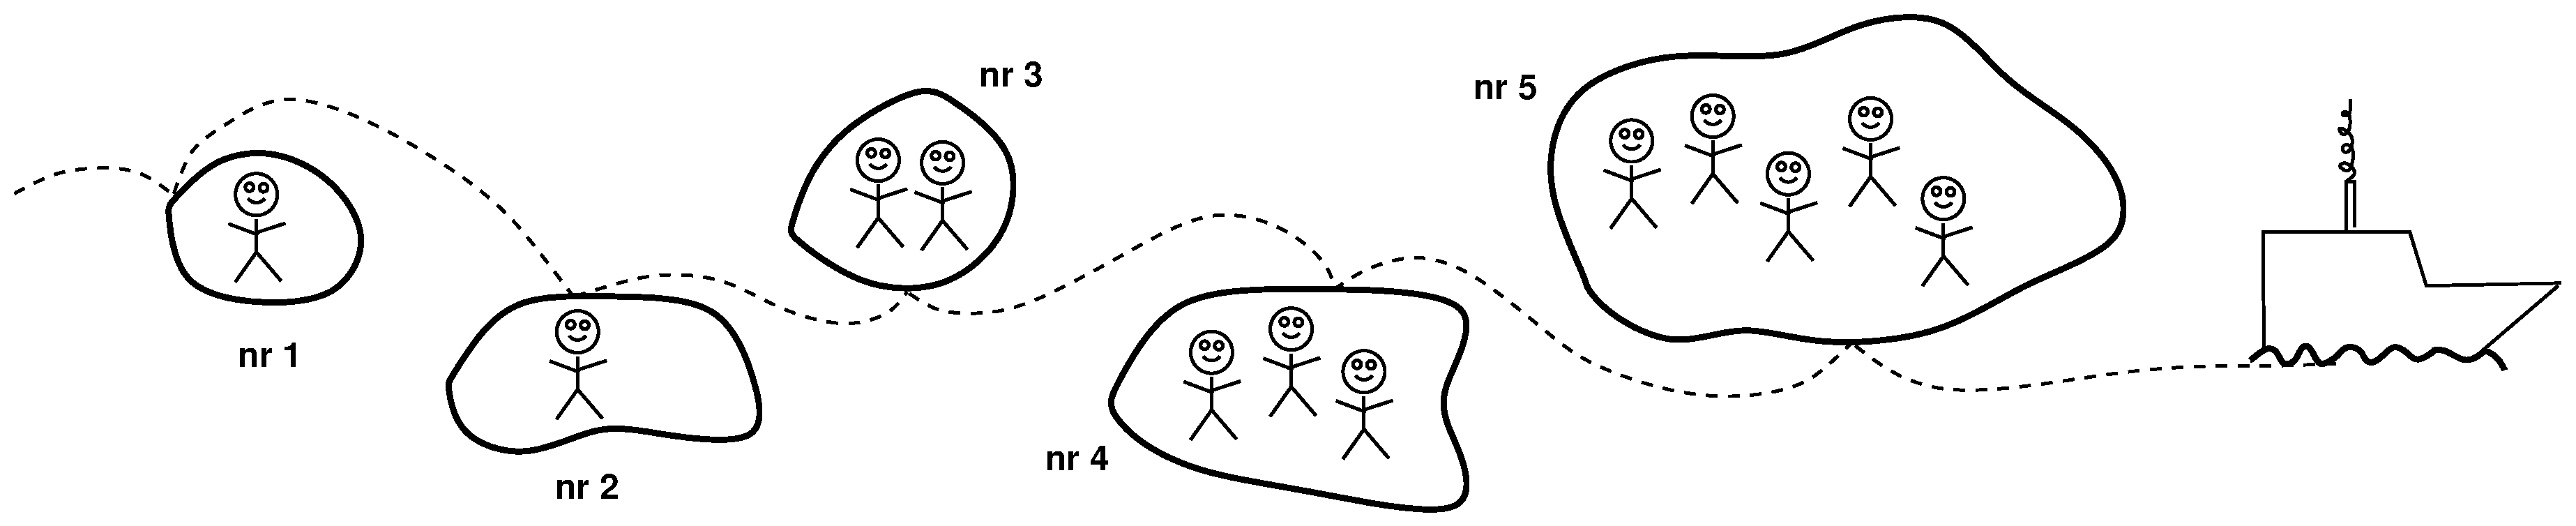
\includegraphics[width=1.0\textwidth]{oarfig}
      \caption{Figuren visar situationen i det första exemplet när den sista (tolfte) deltagaren försvunnit på ö nummer 5.}
\end{figure}
